% Original template by Sebastian Del Bano Rollin, last updated by Oscar Bandtlow February 2024

\includeonly{
    preamble,
    tgv,
    unet,
    tgv_experiment,
}

\documentclass[12pt, oneside]{book}
\usepackage{graphicx}  % this is for includegraphics

\usepackage{setspace}
\onehalfspacing % this sets spacing to 1.5 

\usepackage{amsmath}
\usepackage{amsthm} % for theorems, lemmas etc
\usepackage{amsfonts}
\usepackage{lipsum} % to generate the lipsum random text in the sample

\usepackage{algorithm}
% \usepackage{algpseudocode} % For algorithmic environment
\usepackage{algorithmic}

% \usepackage{biblatex}
\usepackage[%
backend=biber,
natbib=true,
style=apa,
]{biblatex}
\addbibresource{references.bib}


\usepackage[colorlinks=true, urlcolor=blue, pdfborder={0 0 0}]{hyperref}  % For hyperlinks
\hypersetup{
     colorlinks   = true,
     citecolor    = blue
}


\theoremstyle{plain}
\newtheorem{theorem}{Theorem}[section]
\newtheorem{proposition}[theorem]{Proposition}
\newtheorem{lemma}[theorem]{Lemma}
\newtheorem{corollary}[theorem]{Corollary}
\newtheorem{fact}[theorem]{Fact}

\theoremstyle{definition}
\newtheorem{definition}[theorem]{Definition}
\newtheorem{example}[theorem]{Example}
\newtheorem{remark}[theorem]{Remark}
\newtheorem{remarks}[theorem]{Remarks}

\newcommand{\Cov}{\mathrm{Cov}}
\newcommand{\Var}{\mathrm{Var}}

\usepackage{cleveref}
% Configure cleveref to use brackets
\crefformat{figure}{#2[#1]#3}
\crefformat{table}{#2[#1]#3}
\crefformat{equation}{#2(#1)#3}
\crefformat{section}{#2[#1]#3}
\crefformat{subsection}{#2[#1]#3}


\usepackage{tikz}   % for making diagrams
\usetikzlibrary{shapes, arrows.meta, positioning}

\begin{document}


\begin{titlepage}
    \begin{center}
            \vspace{-2cm}
    Data Analytics MSc Dissertation MTHM038, 2023/24
    %Financial Mathematics MSc Dissertation MTHM038, 2022/23
    %Financial Computing MSc Dissertation MTHM038, 2022/23
    %Mathematics MSc Dissertation MMTHM038, 2022/23
            \\
            \Huge
            % \textbf{Constructibility of polygons}
            \textbf{Total Variational Image Denoising with U-Net}
            \\        
            \vspace{0.4cm}
            \LARGE
            With special emphasis on 
            % examples
            experiments
            \\        
            \vspace{0.4cm}        
            \textbf{Thanh Trung Vu, ID ...}% student name and number        
            \\
            \large Supervisor: Dr.\ Kostas Papafitsoros
            \\
            \vspace{0.9cm}
            
\includegraphics[scale=0.25]{QMCrest.jpg}
            \\
            \vspace{0.9cm}        
            \LARGE 
            A thesis presented for the degree of\\
            Master of Science in 
            % \emph{Data Analytics}
            Data Analytics
            \\
            \vspace{0.7cm}        
            \Large
            School of Mathematical Sciences\\ 
            % and \emph{possible joint school}\\
            Queen Mary University of London \\
        \end{center}
    \end{titlepage}
    

\chapter*{Declaration of original work}
\begin{flushright}
This declaration is made on \today.
\end{flushright}


{\bf Student's Declaration:}
I, Thanh Trung Vu, hereby declare that the work in this thesis 
is my original work. I have not copied from any other students' work, 
work of mine submitted elsewhere,  or from any other sources except where due 
reference or acknowledgement is made explicitly in the text. 
Furthermore, no part of this dissertation has been written for me by another person,
by generative artificial intelligence (AI), or by AI-assisted technologies.  
 



Referenced text has been flagged by:
\begin{enumerate}
\item Using italic fonts, {\bf and} % LaTeX: {\it text}  
\item using quotation marks ``\ldots'', {\bf and}
\item explicitly mentioning the source in the text.
\end{enumerate}

%This excludes any definitions known from your modules or that can be found in an undergraduate text book.


\newpage

\thispagestyle{empty}
        \begin{flushright}
                This work is dedicated to my
                grandmothers. 
                % dog 
                % Charles Frederick.
                % Rex.
        \end{flushright}
\vspace{\stretch{2}}\null

\chapter*{Acknowledgements}
I would like to thank my supervisor Dr.\ Kostas Papafitsoros for his guidance and support throughout this project. 
I would also like to thank my family and friends for their encouragement and support.


\chapter*{Abstract}
\lipsum[100]% replace this by your text

\tableofcontents

\chapter{Introduction}
This thesis 

This note presents a conjecture stemming from our investigations in the generation of sigmoid tensor categories of Picard numbers of tori in Banach algebras.
\lipsum[20]
 
\section{Motivation for this work}
In the works of Petri (\cite[Theorem 2.3]{Petri}) we find the following statement

\begin{theorem}[{\cite[Theorem 2.3]{Petri}, see also \cite[pg. 45]{BlackScholes}}]
The Gramm matrix for $E_8$ is:
$$
\begin{pmatrix}
2	&-1&0	&0	&0	&0	&0	&0\\
-1	&2	&-1	&0	&0	&0	&0	&0\\
0	&-1	&2	&-1	&0	&0	&0	&-1\\
0	&0	&-1	&2	&-1	&0	&0	&0\\
0	&0	&0	&-1	&2	&-1	&0	&0\\
0	&0	&0	&0	&-1	&2	&-1	&0\\
0	&0	&0	&0	&0	&-1	&2	&0\\
0	&0	&-1	&0	&0	&0	&0	&2
\end{pmatrix}.
$$
\end{theorem}

\subsection{The problem of exponential extensions}
\lipsum[23]
\subsection{The approach of Junderstein}
\lipsum[23]
\cite{chambolle_pock_2011}

\chapter{Eulerian topological string motives}
\lipsum[23]
\section{Definitions}
\lipsum[23]
\subsection{Tate's theorem}
\paragraph{Preliminary considerations}
\lipsum[23]
\paragraph{Motivic financial algebroids}
\lipsum[23]

\subsection{Grothendieck topologies}
\lipsum[23]

\section{Calculation of the invariant cycles}
\lipsum[23]

\subsection{Fontaine's theorem}
\lipsum[23]

\chapter{Conclusions}
\lipsum[100]

\documentclass{article}
\usepackage{amsmath}
\usepackage{amssymb} % for \mathbb

\usepackage{algorithm}
% \usepackage{algpseudocode} % For algorithmic environment
\usepackage{algorithmic}
\usepackage{hyperref} % For hyperlinks

\usepackage[%
backend=biber,
natbib=true,
style=apa,
]{biblatex}
\addbibresource{references.bib}

\begin{document}

\subsection{Discrete TGV minimisation problem}

Let
\begin{equation}
    \Omega_h = \{(i,j) \mid i,j \in \mathbb{N}, \ 1 \leq i \leq N_1, \ 1 \leq j \leq N_2\}.
\end{equation}
be ...
\newline

An image is a function $\Omega_h \rightarrow \mathbb{R}$. \newline

% A matrix is a discrete function. \newline

Let $u \in \mathbb{R}^{N_1 \times N_2}$ be 
% the image to be reconstructed, 
an image,
$f \in \mathbb{R}^{N_1 \times N_2}$ the observed image. \newline


The spaces of scalar, vector, and symmetric matrix valued functions are defined as (page 13)
\begin{equation}
    \begin{aligned}
    U &= \{u : \Omega_h \rightarrow \mathbb{R}\} \\
    V &= \{u : \Omega_h \rightarrow \mathbb{R}^2\} \\
    W &= \{u : \Omega_h \rightarrow \mathrm{Sym}^2(\mathbb{R}^2)\}
    \end{aligned}
\end{equation}

where $\mathrm{Sym}^2(\mathbb{R}^2)$ is the space of symmetric $2 \times 2$ matrices. \newline

We use the notations $v$ and $w$ where

\begin{equation}
    \begin{aligned}
    $v &\in V$ has components $\left(v\right)^{(1)}$ and $\left(v\right)^{(2)}$ \\
    $w &\in W$ has components $\left(w\right)^{(1,1)}$, $\left(w\right)^{(1,2)}$, $\left(w\right)^{(2,1)}$, $\left(w\right)^{(2,2)} \\
    % & \quad \quad \quad \quad \quad \quad \quad \quad \quad \quad \quad \quad \quad \quad \quad \text{where} \left(w\right)^{(1,2)} = \left(w\right)^{(2,1)}$. 
\end{aligned}
\end{equation}

with \left(w\right)^{(1,2)} = \left(w\right)^{(2,1)}$. \newline

% \begin{equation}
%     a, b : \Omega_h \rightarrow \mathbb{R}, \quad \langle a, b \rangle = \sum_{i=1}^{N_1} \sum_{j=1}^{N_2} a_{i,j} b_{i,j}
% \end{equation}

Use the scalar product notation

\begin{equation}
    a, b : \Omega_h \rightarrow \mathbb{R} : \quad \langle a, b \rangle = \sum_{i=1}^{N_1} \sum_{j=1}^{N_2} a_{i,j} b_{i,j}
\end{equation}

the scalar products in the spaces $V$ and $W$ are

\begin{equation}
\begin{aligned}
    % & u, r \in U:\langle u, r\rangle_U=\left\langle u, r\right\rangle \\
    % u, r \in U &: \langle u, r\rangle_U = \sum_{i=1}^{N_1} \sum_{j=1}^{N_2} u_{i,j} r_{i,j} \\
    v, p \in V &: \langle v, p\rangle_V = \left\langle\left(v\right)^{(1)},\left(p\right)^{(1)}\right\rangle+\left\langle\left(v\right)^{(2)},\left(p\right)^{(2)}\right\rangle \\
    w, q \in W &: \langle w, q\rangle_W = \left\langle\left(w\right)^{(1,1)},\left(q\right)^{(1,1)}\right\rangle+\left\langle\left(w\right)^{(2,2)},\left(q\right)^{(2,2)}\right\rangle+2\left\langle\left(w\right)^{(1,2)},\left(q\right)^{(1,2)}\right\rangle
\end{aligned}
\end{equation}

are the scalar products in $U$, $V$, $W$.
\newline


The $x$ and $y$ forward finite difference operators are (page 13)
\begin{equation}
(\partial_x^+ u)_{i,j} =
\begin{cases}
u_{i+1,j} - u_{i,j} & \text{for } 1 \leq i < N_1 \\
0 & \text{for } i = N_1
\end{cases}
\end{equation}

\begin{equation}
(\partial_y^+ u)_{i,j} =
\begin{cases}
u_{i,j+1} - u_{i,j} & \text{for } 1 \leq j < N_2 \\
0 & \text{for } j = N_2
\end{cases}
\end{equation}

and the backward finite difference operators are (page 13)
\begin{equation}
    (\partial_x^- u)_{i,j} = 
    \begin{cases}
    u_{1,j} & \text{if } i = 1 \\
    u_{i,j} - u_{i-1,j} & \text{for } 1 < i < N_1 \\
    -u_{N_1-1,j} & \text{for } i = N_1
    \end{cases}
\end{equation}
    
\begin{equation}
    (\partial_y^- u)_{i,j} = 
    \begin{cases}
    u_{i,1} & \text{if } j = 1 \\
    u_{i,j} - u_{i,j-1} & \text{for } 1 < j < N_2 \\
    -u_{i,N_2-1} & \text{for } j = N_2
    \end{cases}
\end{equation}






The gradient operator $\nabla_h$ and the symmetrised gradient operator $\mathcal{E}_h$ are defined as (pages 13, 14)

\begin{equation}
    \begin{aligned}
    \nabla_h : U \rightarrow V &, \quad \nabla_h u = 
    \begin{pmatrix}
    \partial_x^+ u \\
    \partial_y^+ u
    \end{pmatrix} \\
    \mathcal{E}_h : V \rightarrow W &, \quad \mathcal{E}_h (v) = 
    \begin{pmatrix}
    \partial_x^- (v)^{(1)} &
    \frac{1}{2} \left( \partial_y^- (v)^{(1)} + \partial_x^- (v)^{(2)} \right) \\
    \frac{1}{2} \left( \partial_y^- (v)^{(1)} + \partial_x^- (v)^{(2)} \right) &
    \partial_y^- (v)^{(2)}
    \end{pmatrix}
    \end{aligned}
\end{equation}

and the divergence operators $\mathrm{div}_h$ are


\begin{equation}
\begin{aligned}
\mathrm{div}_h : V \rightarrow U &, \quad \mathrm{div}_h v = \partial_x^- (v)^{(1)} + \partial_y^- (v)^{(2)} \\
% \end{equation}
% \begin{equation}
\mathrm{div}_h : W \rightarrow V &, \quad \mathrm{div}_h w = 
\begin{pmatrix}
\partial_x^+ (w)^{(11)} + \partial_y^+ (w)^{(12)} \\
\partial_x^+ (w)^{(12)} + \partial_y^+ (w)^{(22)}
\end{pmatrix}
\end{aligned}
\end{equation}

The discrete $\infty\text{-norms}$ are
\begin{equation}
    \begin{aligned}
    v \in V &: \quad \|v\|_\infty = \max_{(i,j) \in \Omega_h} \left( \left( (v)_{i,j}^{(1)} \right)^{2} + \left( (v)_{i,j}^{(2)} \right)^{2} \right)^{1/2} \\
    w \in W &: \quad \|w\|_\infty = \max_{(i,j) \in \Omega_h} \left( \left( (w)_{i,j}^{(1,1)} \right)^{2} + \left( (w)_{i,j}^{(2,2)} \right)^{2} + 2 \left( (w)_{i,j}^{(1,2)} \right)^{2} \right)^{1/2}
\end{aligned}
\end{equation}


Finally, the TGV minimisation problem
is defined as (page ...)
\begin{equation}
    % \min_{u \in L^p(\Omega)} F(u) + \mathrm{TGV}^2_\alpha(u)
    \min_{u \in \mathbb{R}^{N_1 \times N_2}} F(u) + \mathrm{TGV}^2_\alpha(u)
    \label{eq:tgv_minimisation_problem}
\end{equation}

where
the data fidelity/discrepancy function is (page ...)
\begin{equation}
    F(u) = \frac{1}{2} || u - f ||^2_2 = 
    \frac{1}{2}
    % \frac{1}{2 N_1 N_2} 
    \sum_{i=1}^{N_1} \sum_{j=1}^{N_2} (u_{i,j} - f_{i,j})^2
\end{equation}

and
the regularisation term is (page 14)
\begin{equation}
    \mathrm{TGV}^2_\alpha(u) = \max \left\{ \langle u, \mathrm{div}_h v \rangle_U \ \middle| \ 
    \begin{aligned}
    &(v, w) \in V \times W, \ \mathrm{div}_h w = v, \\
    &\|w\|_\infty \leq \alpha_0, \ \|v\|_\infty \leq \alpha_1 
    \end{aligned}
    \right\}
\end{equation}

In [14, 34] it is demonstrated that the TGV functional can be equivalently written as

\begin{equation}
    \text{TGV}^2_{\alpha}(u) = \min_{w \in BD(\Omega)} \alpha_1 \lvert Du - w \rvert (\Omega) + \alpha_0 \lvert \mathcal{E} w \rvert (\Omega),
\end{equation}
    




\subsection{
% PDHG 
Numerical
algorithm for TGV minimisation problem
}

% This minimisation problem is equivalent to the saddle-point problem (page ...).


\begin{algorithm}[H]
    \caption{PDHG algorithm for image denoising with fixed regularisation parameter-map $\boldsymbol{\Lambda}$ (adapted from \cite{kofler2023learning} using the implementation by \cite{dyn_img_pdhg_code})}
    \begin{algorithmic}[1]
    
    \STATE \textbf{Input:} 
    $L = \| [\mathbf{I}, \nabla]^\text{T} \|_2$, 
    % $L = \sqrt{13}$, 
    % $\tau \lesssim 1/L$, 
    % $\sigma \lesssim 1/L$, 
    % $\theta \lesssim 1$, 
    $\tau = \text{sigmoid}(10) / L$, 
    $\sigma = \text{sigmoid}(10) / L$, 
    $\theta = \text{sigmoid}(10)$, 
    noisy image $\mathbf{x}_0$
    
    \STATE \textbf{Output:} reconstructed image $\hat{\mathbf{x}}$
    % \STATE $\mathbf{y} = \mathbf{x}_0$
    \STATE $\bar{\mathbf{x}}_0 = \mathbf{x}_0$
    % \STATE $\mathbf{p}_0 = \mathbf{0}$
    \STATE $\mathbf{p}_0 = \mathbf{x}_0$
    \STATE $\mathbf{q}_0 = \mathbf{0}$
    \FOR{$k < T$}
        % \STATE $\mathbf{p}_{k+1} = \left(\mathbf{p}_k + \sigma ( \bar{\mathbf{x}}_k - \mathbf{y})\right) / (1 + \sigma)$
        \STATE $\mathbf{p}_{k+1} = \left(\mathbf{p}_k + \sigma ( \bar{\mathbf{x}}_k - \mathbf{x}_0)\right) / (1 + \sigma)$
        \STATE $\mathbf{q}_{k+1} = \text{clip}_{\boldsymbol{\Lambda}} \left(\mathbf{q}_k + \sigma \nabla \bar{\mathbf{x}}_k \right)$
        \STATE $\mathbf{x}_{k+1} = \mathbf{x}_k - \tau \mathbf{p}_{k+1} - \tau \nabla^\text{T} \mathbf{q}_{k+1}$
        \STATE $\bar{\mathbf{x}}_{k+1} = \mathbf{x}_{k+1} + \theta (\mathbf{x}_{k+1} - \mathbf{x}_k)$
    \ENDFOR
    \STATE $\hat{\mathbf{x}} = \mathbf{x}_T$
    \end{algorithmic}
    \end{algorithm}


\begin{algorithm}[H]
    \caption{Solve $\min_{u \in U} F_h(u) + \mathrm{TGV}^2_{\alpha}(u)$}

    \begin{algorithmic}[1]
    \STATE \textbf{Input:} $f \in U$, $\alpha_0, \alpha_1 > 0$
    \STATE Choose $\sigma > 0$, $\tau > 0$ such that $\sigma \tau \frac{1}{2} (17 + \sqrt{33}) \leq 1$. Here we choose $\sigma = \tau = 0.29$
    \STATE $u^{[0]} = f$
    \STATE $p^{[0]} = \mathbf{0}_V$
    \STATE $v^{[0]} = \mathbf{0}_V$
    \STATE $w^{[0]} = \mathbf{0}_W$
    \STATE $\bar{u}^{[0]} = u^{[0]}$
    \STATE $\bar{p}^{[0]} = p^{[0]}$

    \FOR {$n = 0, 1, 2, \ldots$}
            \STATE $v^{[n+1]} = \mathcal{P}_{\alpha_1} \left( v^{[n]} + \sigma (\nabla_h \bar{u}^{[n]} - \bar{p}^{[n]}) \right)$
            \STATE $w^{[n+1]} = \mathcal{P}_{\alpha_0} \left( w^{[n]} + \sigma \mathcal{E}_h (\bar{p}^{[n]}) \right)$
            \STATE $u^{[n+1]} = \left( u^{[n]} + \tau (\text{div}_h v^{[n+1]} + f) \right) / ( 1 + \tau )$
            \STATE $p^{[n+1]} = p^{[n]} + \tau (v^{[n+1]} + \text{div}_h w^{[n+1]})$
            \STATE $\bar{u}^{[n+1]} = 2u^{[n+1]} - u^{[n]}$
            \STATE $\bar{p}^{[n+1]} = 2p^{[n+1]} - p^{[n]}$
    \ENDFOR
    \STATE Return $u^{[N]}$ for some large $N$.

    \end{algorithmic}
    \label{alg:pdhg}
\end{algorithm}

where $\mathbf{0}_V \in V$ and $\mathbf{0}_W \in W$ are the zeros matrices in $V$ and $W$ respectively, and $\mathcal{P}_{\alpha_1}$ and $\mathcal{P}_{\alpha_0}$ are the projection operators defined as

\begin{equation}
    \begin{aligned}
    & \mathcal{P}_{\alpha_1}(v) = \frac{v}{\max \left(\mathbf{1}, \frac{1}{\alpha_1}|v|\right)}, \quad v \in V \\
    & \mathcal{P}_{\alpha_0}(w) = \frac{w}{\max \left(\mathbf{1}, \frac{1}{\alpha_0}|w|\right)}, \quad w \in W
    \end{aligned}
\end{equation}



\begin{equation}
    \begin{aligned}
   \quad &|v|_{i,j} = \left( \left( (v)_{i,j}^{(1)} \right)^{2} + \left( (v)_{i,j}^{(2)} \right)^{2} \right)^{1/2} \\
    \quad &|w|_{i,j} = \left( \left( (w)_{i,j}^{(11)} \right)^{2} + \left( (w)_{i,j}^{(22)} \right)^{2} + 2 \left( (w)_{i,j}^{(12)} \right)^{2} \right)^{1/2}
    \end{aligned}
\end{equation}

Here $\mathbf{1}$ is a matrix of ones. 
Note that the division is element-wise.
Denote the matrix underneath as $a$.
The matrix under the division is 2D whereas the matrix above the division is 3D and 4D.
Therefore each element $v_{i,j}^{(k)}$ and $w_{i,j}^{(k,h)}$ of the matrices $v$ and $w$ is divided by the corresponding element $a_{i,j}$ of the matrix under the division.

\newline


This algorithm is used to solve the minimisation problem \ref{eq:tgv_minimisation_problem}.
It is taken from the paper \cite{recovering_piecewise_smooth_multichannel_images}, page ....


%%%%%%%%%%%%%%%%%%%%%%%%%%%%%%%%%%%%%%%%%%%%%%%%%%%%%%%%%%%%%%%%%%

\subsection{Why Projection is dividing by matrix instead of a scalar}


Given matrix $a$, we need to find matrix $u$ such that

\begin{equation}
    u = \arg \min_{|| v ||_\infty \leq 1} || v - a ||_V
\end{equation}

Solution:

Recall that the $L_{1, 2}$-norm is defined as

\begin{equation}
    ||v||_V = \sum_{i,j} \left( \left(v_{i,j}^{(1)}\right)^2 + \left(v_{i,j}^{(2)}\right)^2 \right)^{1/2}
\end{equation}

Constraints:

\begin{equation}
    ||v||_\infty = \max_{(i,j) \in \Omega_h} \left( \left(v_{i,j}^{(1)}\right)^2 + \left(v_{i,j}^{(2)}\right)^2 \right)^{1/2} \leq 1  \quad  \quad  \forall i, j
\end{equation}

or equivalently

\begin{equation}
    \left( \left(v_{i,j}^{(1)}\right)^2 + \left(v_{i,j}^{(2)}\right)^2 \right)^{1/2} \leq 1  \quad  \quad  \forall i, j
\end{equation}


Let $t_{i,j} = \sqrt{(v_{i,j}^{(1)})^2 + (v_{i,j}^{(2)})^2}$.
Then the constraints can be written as

\begin{equation}
    t_{i,j} \leq 1  \quad  \quad  \forall i, j
\end{equation}



We have $n^2$ constraints.
Each constraint is applied to a specific element $v_{i,j}$ and is independent of the others.
Therefore, the solution can be found by solving $n^2$ independent problems:

\begin{equation}
u_{i,j} = \arg \min_{t_{i,j} \leq 1} || v_{i,j} - a_{i,j} ||  \quad \forall i, j
\end{equation}

Denote $v_{i,j} = x$, $a_{i,j} = y$, $u_{i,j} = z$:

\begin{equation}
    z = \arg \min_{|| x ||_2 \leq 1} ||x - y|| \quad \quad \quad x, y, z \in \mathbb{R}^2
\end{equation}

Thus


\begin{equation}
    \begin{aligned}
    z & =
    \begin{cases}
        \frac{y}{||y||_2} & \text{if } ||y||_2 > 1 \\
        % y / ||y||_2 & \text{if } ||y||_2 > 1 \\
        y & \text{if } ||y||_2 < 1 \\
    \end{cases} \\
    & = \frac{y}{\max(\mathbf{1}, ||y||_2)}
    \end{aligned}
\end{equation}



Applying to $u$ and $a$, we have

\begin{equation}
    u_{i,j} = \frac{a_{i,j}}{\max(1, ||a_{i,j}||_2)}
\end{equation}

or in matrix notation,

\begin{equation}
    u = \frac{a}{\max(\mathbf{1}, ||a||_\infty)}
\end{equation}

where $\mathbf{1}$ is a matrix of ones.

TODO: $||a||_\infty$ is a scalar, but we need a matriasdasdx?

% Page 19:
% \begin{equation}
%     (\text{id} + \tau \partial F_h)^{-1}(\bar{u}) =
%     \begin{cases}
%     \frac{\bar{u} + \tau f}{1 + \tau} & \text{if } q = 2, \\
%     f + \mathcal{S}_\tau(\bar{u} - f) & \text{if } q = 1.
%     \end{cases}
% \end{equation}

\printbibliography

\end{document}

\section{Neural Network Architecture}


% Let us first delve into the foundational concept of a convolutional neural network, which underpins the U-Net architecture.



\subsection{
Convolutional Neural Network (CNN)
}

\begin{figure}[H]
    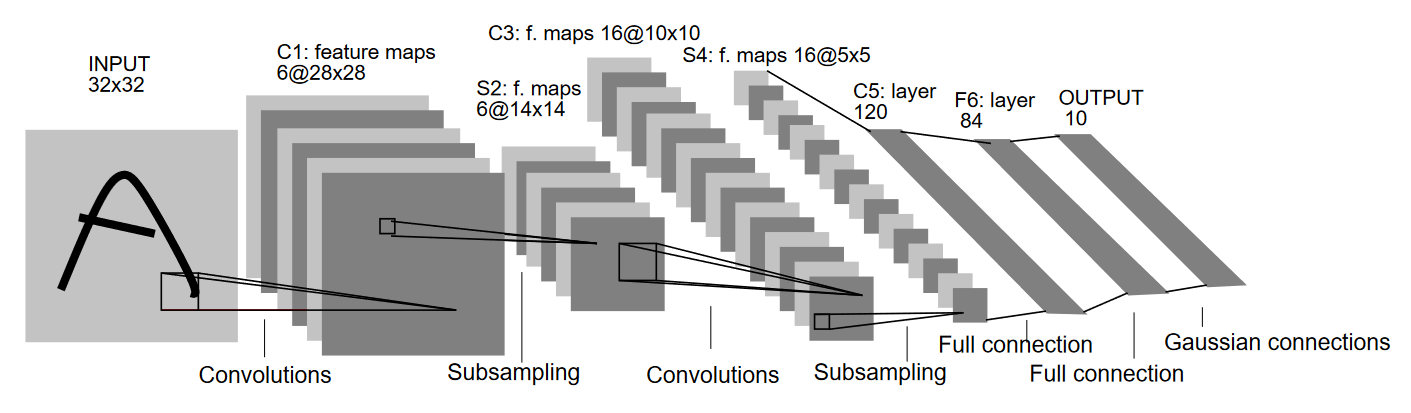
\includegraphics[width=1\linewidth]{../Le-Net 5.png}
    
    \caption{Architecture of LeNet-5, one of the earliest Convolutional Neural Networks (\cite{726791})} 
    \label{fig:lenet}
\end{figure}



Convolutional Neural Networks (CNNs) are a specific type of artificial neural network particularly well-suited for analysing image data and other grid-like patterns. 
Here we assume a 2D CNN architecture, where each layer is represented as one or more 2-dimensional matrices, rather than a vector as in a normal "vanilla" network.
% They excel at tasks like image classification, object detection, and image segmentation. 

% Convolutional Neural Networks (CNNs) are specialised types of artificial neural networks optimised for analysing image data and other grid-like structures. We base our understanding on a two-dimensional (2D) CNN architecture, where each layer is comprised of one or more 2D matrices, in contrast to the vectors used in standard "vanilla" neural networks.

% Here's a breakdown of the key concepts:

% Core Idea:

% CNNs are inspired by the structure and function of the visual cortex in the human brain. The visual cortex processes visual information hierarchically, extracting features from simple edges and shapes to complex objects.

% CNNs achieve similar functionality through convolutional layers and pooling layers. These layers work together to progressively extract and refine features from the input data.

\subsubsection*{Inspiration and Function}



CNNs are inspired by 
% the structure and function of 
the visual cortex in the human brain. 
The visual cortex processes visual information, 
% hierarchically, 
extracting features one-by-one, from simple edges and shapes to complex objects.
CNNs try to mimic this 
% achieve similar functionality 
through convolutional layers and pooling layers. 
% These layers work together to progressively extract and refine features from the input data.

% The design of CNNs draws inspiration from the human visual cortex, which processes visual stimuli by sequentially extracting features, ranging from simple edges and shapes to complex objects. CNNs replicate this hierarchical feature extraction using convolutional layers and pooling layers. 

% Key Components:

    % Convolutional Layers: These layers apply a filter (also called a kernel) to the input data (often an image). The filter slides across the input, computing the dot product between its weights and the corresponding elements in the data. This creates a feature map that highlights specific features the filter is designed to detect.

    % Pooling Layers: These layers downsample the data, reducing its dimensionality while preserving essential features.Pooling techniques like average pooling or max pooling select the most significant value from a local region of the feature map.

    % Activation Functions: CNNs often use activation functions like ReLU (Rectified Linear Unit) after convolutional layers. These functions introduce non-linearity into the network, allowing it to learn complex relationships between features.

    % Fully-Connected Layers: In the later stages of a CNN, fully-connected layers are typically used, similar to regular neural networks. These layers perform classifications or predictions based on the extracted features.


\subsubsection*{Convolutional Layers}

Similar to a normal "vanilla" neural network layer, each element in a convolutional layer's output comes from a linear combination 
% of ...
followed by an activation function.
The difference is the use of filters (also called kernels) instead of a single weight matrix.
Each filter slides across the input, computing the dot product between its weights and the corresponding elements, then passes the output through an activation function.
This is a convolution operation.
For each input matrix, one filter produces one output matrix.
We can have multiple filters in one layer.
Each output matrix is called a feature map, since one filter can be thought of as a feature-extractor that is designed to highlight a specific feature. The number of feature maps is also called the number of channels.
Implementation-wise, using filters instead of weight matrices reduces the ratio between the number of weights and the number of output values, hence cutting down on the number of trainable parameters for 
a image task.
% I have described an example here: [].
% the same amount of output. 


% In a convolutional layer, each output element results from a linear combination of inputs, processed through an activation function—akin to "vanilla" neural networks. However, the critical difference lies in the utilisation of filters (or kernels). Each filter traverses the input matrix, computes the dot product with the corresponding input elements, and channels the result through an activation function. 
% A single filter generates one output matrix, termed a feature map, acting as a feature extractor that emphasises specific characteristics of the input. 
% When multiple filters are employed in a layer, they produce multiple feature maps, with each map corresponding to a different channel. 
% This design significantly reduces the proportion of trainable parameters relative to the number of output values, enhancing efficiency for image-related tasks.

\subsubsection*{Pooling Layers}




An additional type of layer is a pooling layer. Usually we use a max-pooling layer which outputs the maximum instead. This project also utilises max-pooling. The goal is to keep only the most significant values.

These convolutional and pooling layers will form the building block for the U-Net architecture.


% An essential component of CNNs is the pooling layer, typically implemented as a max-pooling layer. This layer simplifies the output by retaining only the maximum values from the defined regions in the feature map. The objective is to preserve the most significant features while reducing data dimensionality. In this project, max-pooling is a crucial technique used to enhance model performance.

% The convolutional and pooling layers constitute the foundational blocks of the U-Net architecture.






\subsection{U-Net Architecture}

The U-Net is a type of neural network that is commonly used for image segmentation (\cite{ronneberger2015unet}).
The U-Net is an encoder-decoder network that is designed to take an image as input and produce a segmentation mask as output.
The U-Net is made up of a series of convolutional layers that downsample the image and a series of transposed convolutional layers that upsample the image.
The U-Net is able to learn to segment images by training on a large dataset of images and their corresponding segmentation masks.


In our case, we will optimise a U-Net model to find the regularisation parameter map 
% $\Lambda_{\Theta}$ 
$\Lambda$ 
that produces the best denoised image for any particular noisy image.


% As previously mentioned, the specific architecture for $\text{NET}_{\Theta}$ is the U-Net, a special type of convolutional neural network architecture.

% An Unrolled Neural Network (U-Net) \cite{ronneberger2015unet} is an extension of a CNN in that we add some so-called skip connections,
% which is similar to the addition connection in a residual network.
% Each skip connection basically concatenates the outputs of two different convolution layers into a bigger output.


% A U-Net, as introduced by Ronneberger et al. \cite{ronneberger2015unet}, extends the conventional CNN architecture by incorporating skip connections, 
% akin to those in a residual network.
% similar to the addition connection in a residual network. 
% These skip connections concatenate the outputs of distinct convolutional layers to generate a larger composite output.
% Each skip connection basically concatenates the outputs of two different convolution layers into a bigger output.

% , in addition to normal pooling layers which condenses the input, we have  which expand the input.

% It has a contracting path (encoder) and an expanding path (decoder) with skip connections in between. 
% This structure is specifically designed for image segmentation, where the network needs to not only extract features but also localise them precisely within the image.

% U-Net are used often in many segmentation tasks, and in recent years have made their ways onto image generation tasks as well.

% \url{https://en.wikipedia.org/wiki/U-Net}: The U-Net architecture stems from the so-called “fully convolutional network” proposed by Long, Shelhamer, and Darrell in 2014. \url{https://arxiv.org/abs/1411.4038}



% The network is based on a fully convolutional neural network[2] whose architecture was modified and extended to work with fewer training images and to yield more precise segmentation.

% The architecture of an unrolled neural network (UNET) is similar to that of an auto-encoder in that it can be viewed as having two parts that are almost opposite-symmetrical.

% Whereas an auto-encoder uses a encoding part and a decoding part, the UNET consists of a contracting path (left side) and an expansive path (right side). 


% The contracting path follows the typical architecture of a convolutional network. 

% It consists of the repeated application of two 3x3 convolutions (unpadded convolutions), each followed by a rectified linear unit (ReLU) and a 2x2 max pooling operation with stride 2 for downsampling. 



% An U-Net can be divided into two main parts, an Encoder and a Decoder. 
% Each part is basically a normal convolution network. The Encoder and Decoder are almost reversely symmetrical. 
The U-Net architecture is divided into two principal components: an Encoder and a Decoder. 

\subsubsection*{Encoder}


The Encoder functions similarly to a standard CNN, utilising a combination of convolutional layers and max-pooling layers organised into distinct "blocks." In this project, each Encoder block comprises a pair of convolutional layers followed by a max-pooling layer, designed to successively double the number of channels (or feature maps) while 
% concurrently 
reducing the feature map size due to the pooling.


% The Encoder is a typical CNN with a combination of convolutional layers and max-pooling layers. The layers are grouped into "blocks". Each encoding block has a few (usually two) convolutional layers followed by one max-pooling layer. In this project we also use blocks of two convolutional layers followed by one max-pooling layer.

% Each successive Encoder block doubles the number of channels (feature maps) while decreasing the size of the feature map due to the pooling operation.

\subsubsection*{Decoder}

% Conversely, the Decoder is structured around a series of blocks that progressively halve the number of channels while enlarging the feature map size, effectively "unrolling" the data. 
% Unlike the Encoder blocks, each Decoder block concludes with an up-convolutional layer followed by a skip connection.
% This up-convolutional layer, essentially a regular convolutional layer, outputs data that is then concatenated with the output from a corresponding Encoder block, facilitating the feature integration across different layers of the network.

The Decoder is also a CNN with a series of blocks. Opposite to an encoding block which doubles the number of channels, each successive decoding block cuts the number of channels (feature maps) in half while increasing the size of the output feature map (hence the "unrolling").
Instead of a max-pooling layer, each decoding block ends with a so-called up-convolutional layer and a skip connection. 
% This up-convolutional layer, essentially a regular convolutional layer, outputs data that is then concatenated with the output from a corresponding Encoder block, facilitating the feature integration across different layers of the network.
The up-convolutional layer is just a normal convolutional layer whose output is concatenated with the output of another convolutional layer in an Encoder block. 
% This concatenation, which increases the size of feature maps instead of decreasing them like a normal CNN would, is where the "unrolling" in the U-Net's name comes from. 




% A U-Net, as introduced by Ronneberger et al. \cite{ronneberger2015unet}, extends the conventional CNN architecture by incorporating skip connections, akin to those in a residual network. These skip connections concatenate the outputs of distinct convolutional layers to generate a larger composite output.



\subsection{Full Architecture}




For this project, our model comprises two primary components:
\begin{enumerate}
    \item A U-Net, denoted as $\text{NET}_{\Theta}$, which is responsible for learning the regularisation parameters $\mathbf{\Lambda}_{\Theta}$ from an input image 
    % $\mathbf{x}_0$
    $\mathbf{x}_{\text{noisy}}$
    \item A Primal Dual Hybrid Gradient (PDHG) algorithm solver 
    % (refer to Appendix), 
    % which utilises both $\mathbf{z}$ and $\mathbf{\Lambda}_{\Theta}$ to transform $\mathbf{x}_0$ into $\hat{\mathbf{x}}
    % $. 
    % This transformation aims to minimise the loss function $L(\mathbf{z}, \mathbf{x})$, thereby facilitating effective reconstruction. 
    % The symbol $\Theta$ represents the set of trainable parameters within the network.
\end{enumerate}

We refer to the set of trainable parameters in the U-Net as $\Theta$, and the output of the U-Net as $\mathbf{\Lambda}_{\Theta}$.

The general architecture is depicted in shown in Figure 1,

\begin{figure}[ht]
  \centering
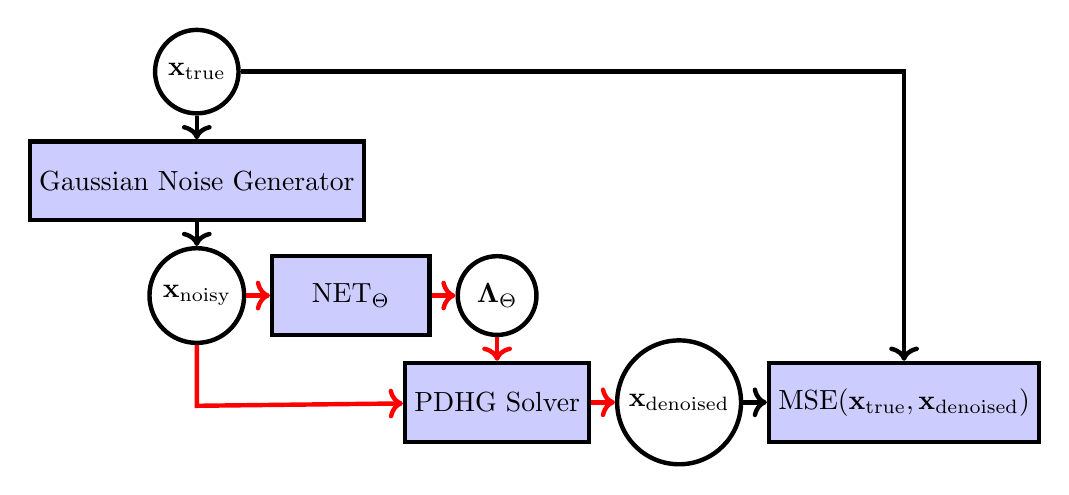
\begin{tikzpicture}[node distance=0.3cm, auto, ultra thick]

  % Define styles for the different layers
  \tikzstyle{output} = [draw, circle, minimum width=1cm, minimum height=1cm]
  \tikzstyle{function} = [draw, rectangle, minimum width=2cm, minimum height=1cm, fill=blue!20]
  \tikzstyle{inference} = [->, ultra thick, red]
  \tikzstyle{normal} = [->, ultra thick, black]

  \node (input) [output] {$\mathbf{x}_{\text{noisy}}$};
  \node (unet) [function, right=of input] {$\text{NET}_{\Theta}$};
  \node (lambda) [output, right=of unet] {$\mathbf{\Lambda}_{\Theta}$};
  \node (pdhg) [function, below=of lambda] {PDHG Solver};
  \node (final_output) [output, right=of pdhg] {$\mathbf{x}_{\text{denoised}}$};   
  \node (noise_generator) [function, above=of input] {Gaussian Noise Generator};
  \node (ground_truth) [output, above=of noise_generator] {$\mathbf{x_{\text{true}}}$};
  \node (loss_function) [function, right=of final_output] {$\text{MSE}(\mathbf{x_{\text{true}}}, \mathbf{x}_{\text{denoised}})$};

  \draw[inference] (input) -- (unet);
  \draw[inference] (unet) -- (lambda);
  \draw[inference] (lambda) -- (pdhg);
  \draw[inference] (pdhg) -- (final_output);
  \draw[inference] (input) -- ++(0, -1.4) -- (pdhg);
  
  \draw[->] (final_output) -- (loss_function);
  \draw[->] (ground_truth) -| (loss_function);
  \draw[->] (ground_truth) -- (noise_generator);
  \draw[->] (noise_generator) -- (input);
%   \draw[->] (loss_function) -- ++(0, -1) -| (unet);

\end{tikzpicture}

\caption{The general architecture 
% \caption{Training 
% of PDHG Net 
% \cite{kofler2023learning}
}

\label{fig:training}
\end{figure}

where
\begin{itemize}
    \item $\mathbf{x_{\text{true}}}$ represents the clean image, serving as the ground truth.
    \item $\mathbf{x_{\text{noisy}}}$ denotes the noisy image inputted to $\text{NET}_{\Theta}$.
    \item $\mathbf{\Lambda}_{\Theta}$ is the regularisation parameters map which is the final output from the U-Net. 
    % Throughout this project, $\mathbf{\Lambda}$ and $\mathbf{\Lambda}_{\Theta}$ are used interchangeably.
\end{itemize}

We can treat the PDHG solver as the final hidden layer in our network. 
The result of the loss function $\text{MSE}(\mathbf{x_{\text{true}}}, \mathbf{x_{\text{denoised}}})$ 
is then used for backpropagation to train the parameters $\Theta$.



% \begin{figure}[ht]
% \hspace*{-0.5cm} % Adjust the value as needed
% \begin{tikzpicture}[node distance=0.3cm, auto, ultra thick, transform shape, shift={(-10cm,0)}]
%     % Define styles
%     \tikzstyle{rec16_1} = [draw, rectangle, minimum width=0.1cm, minimum height=2cm, fill=blue!30]
%     \tikzstyle{rec16} = [draw, rectangle, minimum width=0.6cm, minimum height=2cm, fill=blue!30]
%     \tikzstyle{rec32} = [draw, rectangle, minimum width=1.2cm, minimum height=1cm, fill=blue!30]
%     \tikzstyle{rec64} = [draw, rectangle, minimum width=2.0cm, minimum height=0.5cm, fill=blue!30]
%     \tikzstyle{rec64_2} = [draw, rectangle, minimum width=2.0cm, minimum height=0.5cm, fill=blue!30]
%     \tikzstyle{rec2} = [draw, rectangle, minimum width=0.4cm, minimum height=2cm, fill=blue!30]
%     \tikzstyle{rec_white32} = [draw, rectangle, minimum width=1.2cm, minimum height=1cm, fill=white]
%     \tikzstyle{rec_white16} = [draw, rectangle, minimum width=0.6cm, minimum height=2cm, fill=white]
%     \tikzstyle{normalconv} = [->, ultra thick, blue]
%     \tikzstyle{maxpool} = [->, ultra thick, red]
%     \tikzstyle{upconv} = [->, ultra thick, green]
%     \tikzstyle{finalconv} = [->, ultra thick, black]

%     % ENCODER
%     \node (en1_input) [rec16_1] {};
%     \node (en1con1_output) [rec16, right=of en1_input] {};
%     \node (en1con2_output) [rec16, right=of en1con1_output] {};

%     \node (en2_input) [rec32, below=of en1con2_output] {};
%     \node (en2con1_output) [rec32, right=of en2_input] {};
%     \node (en2con2_output) [rec32, right=of en2con1_output] {};

%     \node (en3_input) [rec64, below=of en2con2_output] {};
%     \node (en3con1_output) [rec64, right=of en3_input] {};
%     \node (en3con2_output) [rec64, right=of en3con1_output] {};
%     \node (upcon1_input) [rec64_2, right=of en3con2_output] {};

%     % DECODER
%     \node (de1_input) [rec32, above=of upcon1_input] {};
%     \node (skip1_output) [rec_white32, left=0cm of de1_input] {};
%     \node (de1con1_output) [rec32, right=of de1_input] {};
%     \node (de1con2_output) [rec32, right=of de1con1_output] {};

%     \node (de2_input) [rec16, above=of de1con2_output] {};
%     \node (skip2_output) [rec_white16, left=0cm of de2_input] {};
%     \node (de2con1_output) [rec16, right=of de2_input] {};
%     \node (de2con2_output) [rec16, right=of de2con1_output] {};

%     % Final output layer
%     \node (final_output) [rec2, right=of de2con2_output] {};

%     % CONNECTIONS
%     \draw[normalconv] (en1_input) -- (en1con1_output);
%     \draw[normalconv] (en1con1_output) -- (en1con2_output);
%     % \draw[maxpool] (en1con2_output) -- ++(0,-0.5) -| (en2_input);
%     \draw[maxpool] (en1con2_output) -- (en2_input);
    
%     \draw[normalconv] (en2_input) -- (en2con1_output);
%     \draw[normalconv] (en2con1_output) -- (en2con2_output);
%     % \draw[maxpool] (en2con2_output) -- ++(0,-0.5) -| (en3_input);
%     \draw[maxpool] (en2con2_output) -- (en3_input);
    
%     \draw[normalconv] (en3_input) -- (en3con1_output);
%     \draw[normalconv] (en3con1_output) -- (en3con2_output);
%     \draw[maxpool] (en3con2_output) -- (upcon1_input);
    
%     % \draw[upconv] (en3con2_output) -- ++(0,0.5) -| (de1_input);
%     \draw[upconv] (upcon1_input) -- (de1_input);
%     \draw[normalconv] (de1_input) -- (de1con1_output);
%     \draw[normalconv] (de1con1_output) -- (de1con2_output);
    
%     % \draw[upconv] (de1con2_output) -- ++(0,0.5) -| (de2_input);
%     \draw[upconv] (de1con2_output) -- (de2_input);
%     \draw[normalconv] (de2_input) -- (de2con1_output);
%     \draw[normalconv] (de2con1_output) -- (de2con2_output);
    
%     \draw[finalconv] (de2con2_output) -- (final_output);

%     % Skip connections
%     \draw[->, dashed, ultra thick] (en2con2_output.east) -- ++(0.5,0) |- (skip1_output.west);
%     \draw[->, dashed, ultra thick] (en1con2_output.east) -- ++(0.5,0) |- (skip2_output.west);

% \end{tikzpicture}
% \caption{Our $\text{NET}_{\Theta}$ Architecture}
% \label{fig:my_unet}
% \end{figure}


\begin{figure}[ht]
  \includegraphics[width=1\linewidth]{../../../PlotNeuralNet/unet-true-voice-32/unet-visualisation-true-voice-32.pdf}
  % \includegraphics[width=1\linewidth]{images/unet-visualisation-true-voice-32.pdf}
\caption{Our $\text{NET}_{\Theta}$ Architecture}
\label{fig:my_unet}
\end{figure}


% Conversely, the Decoder incorporates two decoding blocks, one fewer than the Encoder. This configuration deviates from some common implementations where the number of encoding and decoding blocks are equal, and a "bottle-neck" comprising two additional convolutional layers is placed between them. In our model, we treat the final block of the Encoder as this bottle-neck. The first decoding block in the Decoder reduces the number of channels back to 32, and the second further reduces them to 16.

% Similarly we have three decoding blocks.
% Each decoding block in our model concludes with an up-convolutional layer, which serves the same function as a typical convolutional layer, followed by a skip connection. The first skip connection takes the 32-channel output from the second encoding block and merges it with the 32-channel output from the first up-convolutional layer. This combination produces a 64-channel output, which is then processed by the first decoding block. The second skip connection similarly merges the 16-channel output from the first encoding block with the 16-channel output from the second up-convolutional layer, resulting in a 32-channel input for the second decoding block.

% The final stage in our architecture employs a convolutional layer to convert the 16-channel output from the last decoding block into a 2-channel output, thus producing two matrices as the ultimate output of our model.



\subsection{Results}

\appendix
\chapter{Implementation of the {\tt BarrierOptionCVA} class}
\lipsum[100]
\chapter[Shorter running title]{Additional details on the Gundermanian determinant}
\lipsum[100]


\printbibliography


% \bibliographystyle{plain}
% \begin{thebibliography}{OOO}
% \bibitem[P99]{Petri}
%    William Petri, 
%   {\it Analysis of infinitely generated frog complexes},
% 	Rendicoti Ran\ae \ Analysorum, 234 {\bf (4)}, 34--21, 2015

% \bibitem[Ross]{Ross}
%   Sheldon Ross, {\it An Elementary Introduction to Mathematical Finance},
% 	3rd Edition, Cambridge University Press, 2011
	
% \bibitem[Hull]{Hull}
% 	John C. Hull, 
% 	{\it Options, Futures, and Other Derivatives},
% 	8th Edition, Pearson Education, 2011

% \bibitem[BS]{BlackScholes}
% 	Fischer Black and  Myron Scholes,
% 	{\it \href{https://www.cs.princeton.edu/courses/archive/fall09/cos323/papers/black_scholes73.pdf}
% 	{The Pricing of Options and Corporate Liabilities}},
% 	Journal of Political Economy 81 {\bf 3}, 637--654,  (1973)
	
% \end{thebibliography}










\end{document}
